\documentclass{article}
\usepackage[margin=3cm]{geometry}
\usepackage[utf8]{inputenc}
\usepackage{amsmath}
\usepackage{amssymb}
\usepackage{float}
\usepackage{enumitem}
\usepackage{graphicx}
\usepackage{caption}
\usepackage{subcaption}

\graphicspath{ {plots/} }

\title{Nonlinear Optimization - Homework 4}
\author{Christian Segercrantz 481056}


\begin{document}
	\maketitle
	\pagebreak
\section*{4.1 Frank-Wolfe Method}
	The completed code can be seen from the attached file. Compared to the pseudo code found in the lecture slides, the algorithm did not result in the correct answer when using $\nabla f(x)^\top d^k$ but when using $\nabla f(x)^\top x$ as the objective value. At the first iteration $d^k=x$ since $x^k=0$, but from there this result seems odd. Using $d^k$ results in way faster convergence, but another optimal value.
\section*{4.2 Interior-Point Method for Quadratic Problems}
	The problem
	\begin{alignat}{2}
		\text{min. } & c^\top x + \frac{1}{2}x^\top Q x \\
		\text{subject to: } & Ax = b \label{eq:4.1_g1_primal}\\
		&x \geq 0
	\end{alignat}
	and it's dual
	\begin{alignat}{2}
		\text{min. } & b^\top v \frac{1}{2}x^\top Q x \\
		\text{subject to: } & A^\top v + u - Qx = c \label{eq:4.1_g1_dual}\\
		&x \geq 0.
	\end{alignat}
\subsection*{a)}
	The KKT conditions for the problem are
	\begin{align}
		0=& \nabla f(x) + \sum_j u_j \nabla g(x) + \sum_i v_i\nabla h(x) \\
		u_jg(x) =& 0 \quad j=1...m \\
		v_ih(x) =& 0 \quad i=1...l \\
		x\in X, g_j(x)\leq& 0 \quad j=1...m \\
		u_j\geq& 0 \quad j=1...m \\
	\end{align}
	which for our problem becomes
	\begin{align}
		\nabla (c^\top x + \frac{1}{2}x^\top Q x) - u_1 + v_1 \nabla(Ax-b) =& 0\\
		c^\top+Qx - u_1 + v_1A =& 0 \\
		u_1^\top x =& 0 \\
		v_1(Ax-b) =& 0  \\
		x \geq& 0 \\
		u_i\geq& 0  \\
	\end{align}
\subsection*{b)}
	The general form of the Barrier problem looks as
	\begin{alignat}{2}
		\text{(BP): } & \inf_\mu \theta(\mu) \\
		\text{subject to: } & \mu > 0\\
	\end{alignat}
	where $\theta(\mu)$ is, in our case,
	\begin{align}
		\theta(\mu)=& \inf_x \{ f(x) + \mu B(x): -x \leq 0\}\\
		=& \inf_x \{ f(x) + \mu (-\sum_{j=1}^{m}\ln(-g_j(x))): -x \leq 0\} \\
		=& \inf_x \{ f(x) + \mu (-\ln(x)): -x \leq 0\} \\
		=& \inf_x \{ f(x) - \mu \ln(x): -x \leq 0\}.
	\end{align} 
	The problem can thus be formulated as
	\begin{alignat}{2}
		\text{(BP): } & \inf_\mu \{\inf_x \{ c^\top x + \frac{1}{2}x^\top Q x - \mu \ln(x): -x \leq 0\}\} \\
		\text{subject to: } & \mu > 0.
	\end{alignat}
\subsection*{c)}
	The first part of the KKT conditions of part b) is
	\begin{align}
		c^\top+Qx - u_1 + v_1A -\frac{\mu}{x} &= 0
	\end{align}
	and the rest follows as from the a) part.
	
	From the lecture slides and using our problem we get the following Newton system
	\begin{equation}
		\begin{bmatrix}
			A & 0 & 0\\
			-Q & A^\top & I\\
			\bar{U}^k & 0 & \bar{X}^k
		\end{bmatrix}
		\begin{bmatrix}
			d_x^{k+1}\\
			d_v^{k+1}\\
			d_u^{k+1}
		\end{bmatrix} =
		\begin{bmatrix}
			Ax^{k}-b \\
			A^\top v^k+ u^k -Qx^k-c\\
			X^k U^k e - \mu^{k+1}e
		\end{bmatrix} = -
		\begin{bmatrix}
			r_p\\
			r_d\\
			r_c
		\end{bmatrix},
	\end{equation}
	where the first row of the matrix after the first equality sign is the condition of the primal problem and the second is the condition of the dual problem. From this we get the following system of equations
	\begin{equation}
		\begin{cases}
			Ad_x^{k+1} = Ax^{k}-b = -r_p \\
			-Qd_x^{k+1}+A^\top d_v^{k+1} + Id_u = A^\top v^k+ u^k -Qx^k-c = -r_d\\
			\bar{U}^kd_x + \bar{X}^kd_u= X^k U^k e - \mu^{k+1}e = -r_c
		\end{cases}.
	\end{equation}
	From the second expression we can solve $d_u$ as 
	\begin{align}
		A^\top d_v^{k+1} + Id_u &= -r_d\\
		d_u &= -r_d +Qd_x^{k+1}- A^\top d_v^{k+1}.
	\end{align}
	By substituting this into third expression we get
	\begin{align}
		\bar{U}^kd_x + \bar{X}^kd_u &= -r_c\\
		\bar{U}^kd_x - \bar{X}^k(r_d -Qd_x^{k+1} + A^\top d_v^{k+1}) &= -r_c\\
		\bar{U}^kd_x + \bar{X}^kQd_x^{k+1} - \bar{X}^kr_d -\bar{X}^kA^\top d_v^{k+1} &= -r_c\\
		(\bar{U}^k + \bar{X}^kQ)d_x^{k+1} &= -r_c + \bar{X}^kr_d +\bar{X}^kA^\top d_v^{k+1}\\
		d_x^{k+1} &= (\bar{U}^k - \bar{X}^kQ) ^{-1}(-r_c + \bar{X}^kr_d +\bar{X}^kA^\top d_v^{k+1}) \label{eq:d_x}
	\end{align}
	From the first expression we know that	$Ad_x^{k+1}  = -r_p$, thus by multiplying the Equation \ref{eq:d_x} by $A$ we get that 
	\begin{equation}
		Ad_x^{k+1} = A(\bar{U}^k + \bar{X}^kQ) ^{-1}(-r_c + \bar{X}^kr_d + \bar{X}^kA^\top d_v^{k+1}) = -r_p
	\end{equation}
	from which we can solve $d_v^{k+1}$ as 
	\begin{align}
		-r_p &= A(\bar{U}^k + \bar{X}^kQ)^{-1}(-r_c + \bar{X}^kr_d +\bar{X}^kA^\top d_v^{k+1})\\
		-r_p &= -A(\bar{U}^k + \bar{X}^kQ)^{-1}r_c + A(\bar{U}^k + \bar{X}^kQ)^{-1}\bar{X}^kr_d +A(\bar{U}^k + \bar{X}^kQ)^{-1}\bar{X}^kA^\top d_v^{k+1}\\
		A(\bar{U}^k + \bar{X}^kQ)^{-1}\bar{X}^kA^\top d_v^{k+1} &= -r_p + A(\bar{U}^k + \bar{X}^kQ)^{-1}r_c - A(\bar{U}^k + \bar{X}^kQ)^{-1}\bar{X}^kr_d	\\
 		d_v^{k+1} &= (A(\bar{U}^k + \bar{X}^kQ)^{-1}\bar{X}^kA^\top)^{-1}(-r_p + A(\bar{U}^k + \bar{X}^kQ)^{-1}r_c - A(\bar{U}^k + \bar{X}^kQ)^{-1}\bar{X}^kr_d)	\\
 		d_v^{k+1} &= (A(\bar{U}^k + \bar{X}^kQ)^{-1}\bar{X}^kA^\top)^{-1}(-r_p + A(\bar{U}^k + \bar{X}^kQ)^{-1}(r_c - Xr_d))	
	\end{align}
	We know how a solution for $d_v^{k+1}$ which we can substitute into the earlier expressions for $d_x^{k+1} $ and $ d_u^{k+1}$. The trajectory of the algorithm can be seen in Figure \ref{fig:2d}.
\subsection*{d)}
	Using the provided skeleton and earlier results, we obtain the solution $x\approx\begin{bmatrix}0.905 & 0.819\end{bmatrix}^\top$ after 6 iterations. 
	\begin{figure}[H]
		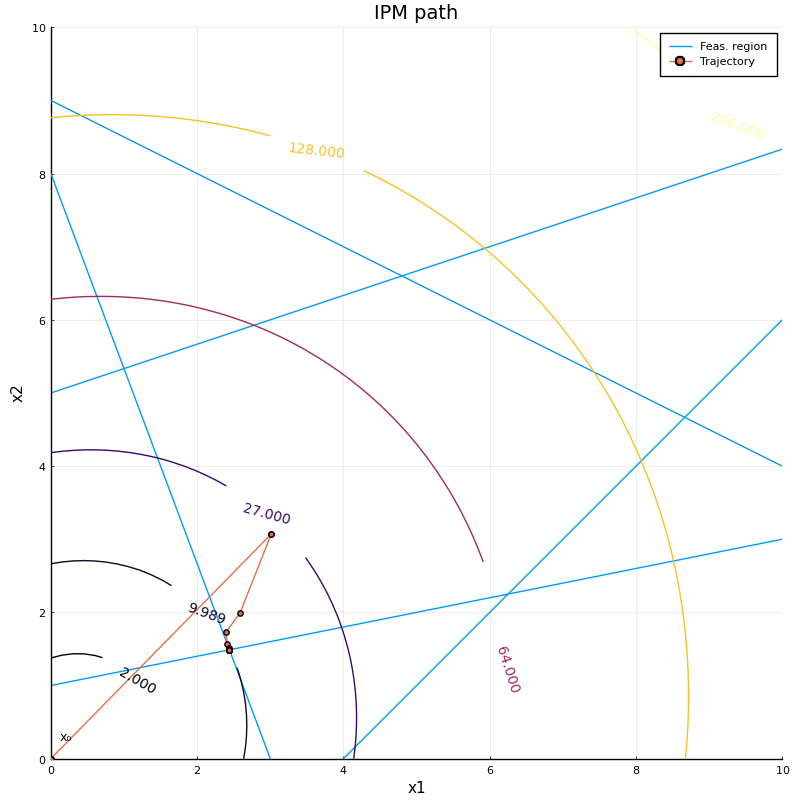
\includegraphics[width=0.8\textwidth]{qp_convergence.png}
		\caption{The trajectory the x-values gotten from the interior-point method algorithm used.}
		\label{fig:2d}
	\end{figure}
\section*{4.3 Sequential Quadratic Programming}
	\subsection*{a)}
	Using the skeleton and lecture notes 11 we can create the algorithm. The algorithm can be seen in the attached file. It seems using the default values for the trust region $\Delta$ and the penalty term $\mu$ seem to be enough for the algorithm to converge. The plot is made using the default values. Some additional values were tested, e.g. $\Delta=0.5$ and $\mu=1$ did not result in convergence while very large values $\Delta=1000$ and $\mu=1000$ did result in convergence. Plots of the aforementioned examples can be seen in Figure \ref{fig:3_extra}. We can see that the default values seem to provide the best result.
	\subsection*{b)}
	\begin{figure}[H]
		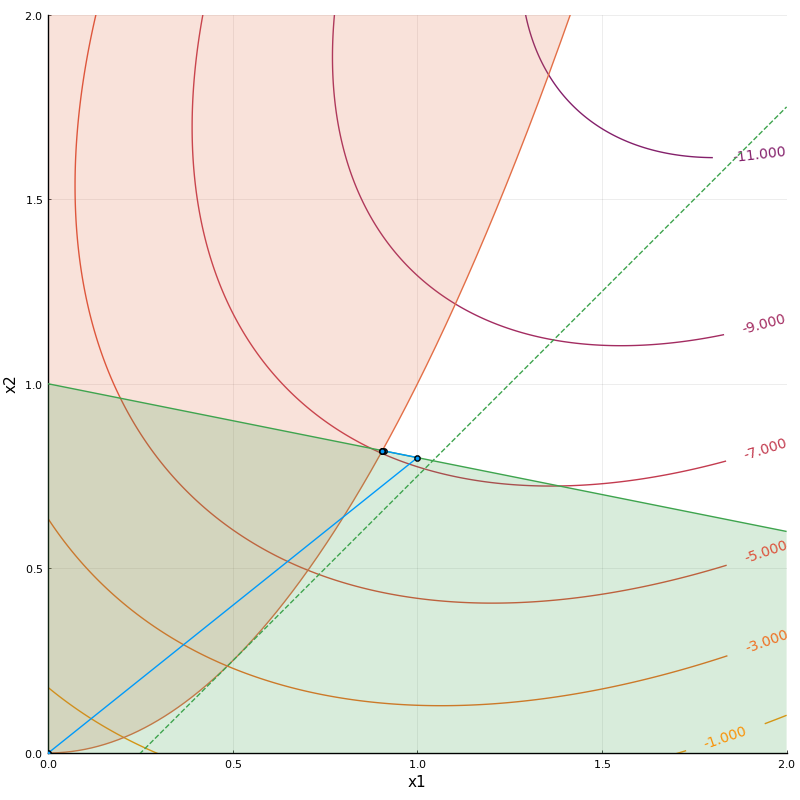
\includegraphics[width=0.8\textwidth]{SQP_example.png}
		\caption{The trajectory the x-values take, gotten from the interior-point method algorithm used. The feasible area is also highlighted}
		\label{fig:3b}
	\end{figure}
	\begin{figure}
		\centering
		\begin{subfigure}[b]{0.45\textwidth}
			\centering
			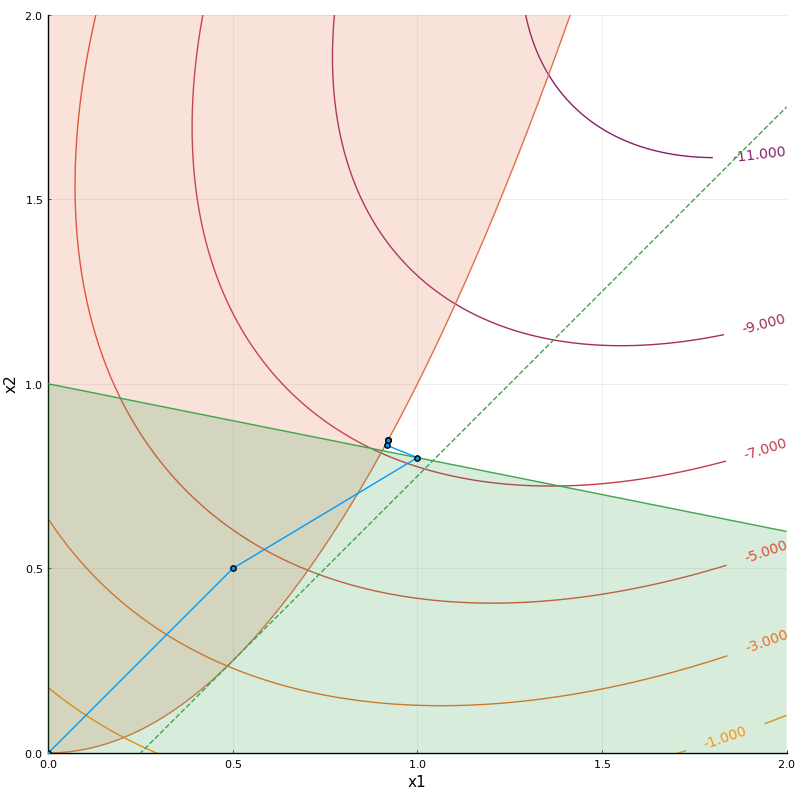
\includegraphics[width=\textwidth]{SQP_example_small}
			\caption{$\Delta=0.5$, $\mu=1$}
		\end{subfigure}
		\hfill
		\begin{subfigure}[b]{0.45\textwidth}
			\centering
			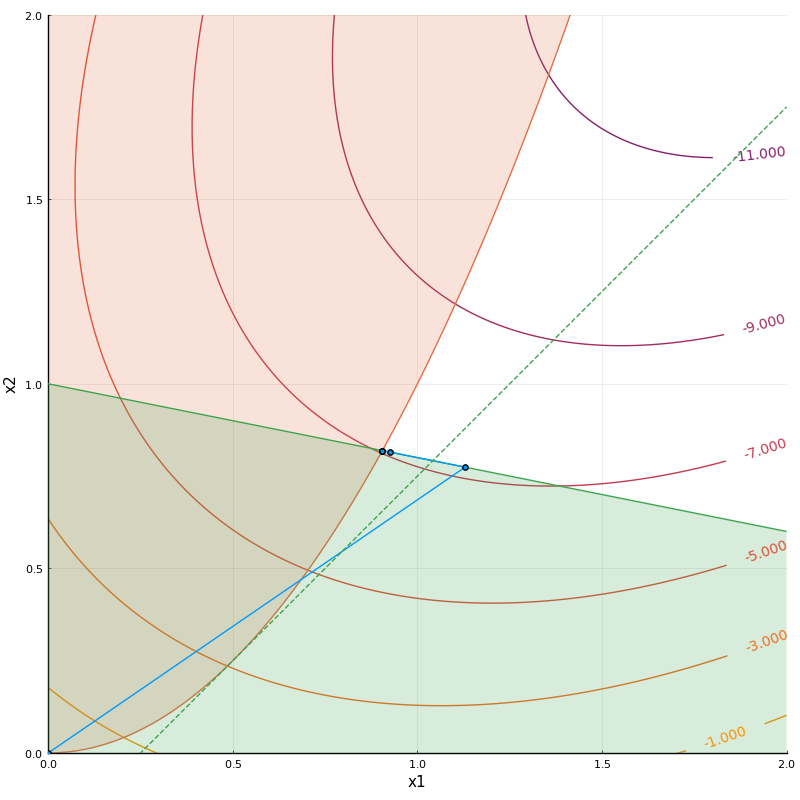
\includegraphics[width=\textwidth]{SQP_example_large}
			\caption{$\Delta=1000$, $\mu=1000$}
		\end{subfigure}
		\caption{Trejectory plots of alternative trust region $\Delta$ and the penalty term $\mu$ values.}
		\label{fig:3_extra}
	\end{figure}
\end{document}